\documentclass{jcgt}

\usepackage{amsmath}
\usepackage{listings}
\usepackage{xcolor}
\usepackage[normalem]{ulem}
\usepackage{siunitx}
\usepackage{csquotes}
\usepackage{url}
\usepackage{subcaption}
\usepackage{xcolor}
\usepackage{algorithm}
\usepackage{algorithmicx}
\usepackage{algpseudocode}
\usepackage{mathtools}
\usepackage{xfrac}
\usepackage{comment}
\usepackage{natbib}
\usepackage[font={small,it}]{caption}
\usepackage{tikz}
\usetikzlibrary{positioning}

\usepackage[export]{adjustbox}

\setciteauthor{Matthias Raab and Laurent Belcour and Frankie Liu and Jamie Portsmouth}
\setcitetitle{The Minimal Retroreflective Microfacet Model (MRM)}
%\setheadtitle{Abbreviated title, only if full title won't fit in page headers}

% Mark submissions with the date of submission using the following line:
\submitted{\today}

% Once an article is accepted accepted, switch to the following line and comment the preceding one. The editor will supply the argument values.
%\accepted{yyyy-mm-dd}{yyyy-mm-dd}{yyyy-mm-dd}{Editor Name}{volume}{issue}{1}{6}{yyyy}
\seturl{http://jcgt.org/published/vol/issue/num/}
\newcommand{\vecv}{\mathbf{v}}
\newcommand{\vecvv}{\mathbf{v'}}
\newcommand{\vecl}{\mathbf{l}}
\newcommand{\vecll}{\mathbf{l'}}
\newcommand{\vecn}{\mathbf{n}}
\newcommand{\vecm}{\mathbf{m}}
\newcommand{\vech}{\mathbf{h}}
\newcommand{\vechr}{\mathbf{h_r}}
\newcommand{\vecht}{\mathbf{h_t}}
\newcommand{\vecb}{\mathbf{b}}
\newcommand{\vecbr}{\mathbf{b_r}}
\newcommand{\vecbt}{\mathbf{b_t}}
\newcommand{\vecx}{\mathbf{x}}
\newcommand{\vecxx}{\mathbf{x'}}
\newcommand{\vecy}{\mathbf{y}}
\newcommand{\vecyy}{\mathbf{y'}}
\newcommand{\etav}{\eta_{\mathbf{v}}}
\newcommand{\etal}{\eta_{\mathbf{l}}}
\newcommand{\etax}{\eta_{\mathbf{x}}}
\newcommand{\etay}{\eta_{\mathbf{y}}}
\newcommand{\vdot}[2]{#1 \cdot #2}
%\newcommand{\vdot}[2]{#1\cdot#2}
\newcommand{\avdot}[2]{\lvert\vdot{#1}{#2}\rvert}
\newcommand{\cldot}[2]{\langle #1 , #2 \rangle}

\newcommand{\diff}{\, \mathrm{d}}

\newcommand{\laurent}[1]{{\color{blue}\textbf{[Laurent:} #1\textbf{]}}}

\includecomment{introduction}
\includecomment{existing-models}
\includecomment{eon}
\includecomment{eon-sampling}
\includecomment{conclusion}

\urlstyle{same}

\captionsetup[table]{skip=10pt}

\lstdefinestyle{snippet}{
  float=tp,
  floatplacement=tbp,
  abovecaptionskip=5pt
}

\lstdefinelanguage{GLSL}%
{%
	morekeywords={%
	% HLSL constants
		false,FALSE,NULL,true,TRUE,%
	% GLSL predefinde macro constant
		__LINE__,__FILE__,__VERSION__,GL_core_profile,GL_es_profile,GL_compatibility_profile,%
	% GLSL precision modifier
		precision,highp,mediump,lowp,%
	% GLSL types
		void,bool,int,uint,float,double,vec2,vec3,vec4,dvec2,dvec3,dvec4,bvec2,bvec3,bvec4,ivec2,ivec3,ivec4,uvec2,uvec3,uvec4,mat2,mat3,mat4,mat2x2,mat2x3,mat2x4,mat3x2,mat3x3,mat3x4,mat4x2,mat4x3,mat4x4,dmat2,dmat3,dmat4,dmat2x2,dmat2x3,dmat2x4,dmat3x2,dmat3x3,dmat3x4,dmat4x2,dmat4x3,dmat4x4,sampler1D,sampler2D,sampler3D,image1D,image2D,image3D,samplerCube,imageCube,sampler2DRect,image2DRect,sampler1DArray,sampler2DArray,image1DArray,image2DArray,samplerBuffer,imageBuffer,sampler2DMS,image2DMS,sampler2DMSArray,image2DMSArray,samplerCubeArray,imageCubeArray,sampler1DShadow,sampler2DShadow,sampler2DRectShadow,sampler1DArrayShadow,sampler2DArrayShadow,samplerCubeShadow,samplerCubeArrayShadow,isampler1D,isampler2D,isampler3D,iimage1D,iimage2D,iimage3D,isamplerCube,iimageCube,isampler2DRect,iimage2DRect,isampler1DArray,isampler2DArray,iimage1DArray,iimage2DArray,isamplerBuffer,iimageBuffer,isampler2DMS,iimage2DMS,isampler2DMSArray,iimage2DMSArray,isamplerCubeArray,iimageCubeArray,atomic_uint,usampler1D,usampler2D,usampler3D,uimage1D,uimage2D,uimage3D,usamplerCube,uimageCube,usampler2DRect,uimage2DRect,usampler1DArray,usampler2DArray,uimage1DArray,uimage2DArray,usamplerBuffer,uimageBuffer,usampler2DMS,uimage2DMS,usampler2DMSArray,uimage2DMSArray,usamplerCubeArray,uimageCubeArray,struct,%
	% GLSL support variables
		gl_BackColor,gl_BackLightModelProduct,gl_BackLightProduct,gl_BackMaterial,gl_BackSecondaryColor,gl_ClipDistance,gl_ClipPlane,gl_ClipVertex,gl_Color,gl_DepthRange,gl_DepthRangeParameters,gl_EyePlaneQ,gl_EyePlaneR,gl_EyePlaneS,gl_EyePlaneT,gl_Fog,gl_FogCoord,gl_FogFragCoord,gl_FogParameters,gl_FragColor,gl_FragCoord,gl_FragData,gl_FragDepth,gl_FrontColor,gl_FrontFacing,gl_FrontLightModelProduct,gl_FrontLightProduct,gl_FrontMaterial,gl_FrontSecondaryColor,gl_InstanceID,gl_Layer,gl_LightModel,gl_LightModelParameters,gl_LightModelProducts,gl_LightProducts,gl_LightSource,gl_LightSourceParameters,gl_MaterialParameters,gl_ModelViewMatrix,gl_ModelViewMatrixInverse,gl_ModelViewMatrixInverseTranspose,gl_ModelViewMatrixTranspose,gl_ModelViewProjectionMatrix,gl_ModelViewProjectionMatrixInverse,gl_ModelViewProjectionMatrixInverseTranspose,gl_ModelViewProjectionMatrixTranspose,gl_MultiTexCoord0,gl_MultiTexCoord1,gl_MultiTexCoord2,gl_MultiTexCoord3,gl_MultiTexCoord4,gl_MultiTexCoord5,gl_MultiTexCoord6,gl_MultiTexCoord7,gl_Normal,gl_NormalMatrix,gl_NormalScale,gl_ObjectPlaneQ,gl_ObjectPlaneR,gl_ObjectPlaneS,gl_ObjectPlaneT,gl_Point,gl_PointCoord,gl_PointParameters,gl_PointSize,gl_Position,gl_PrimitiveIDIn,gl_ProjectionMatrix,gl_ProjectionMatrixInverse,gl_ProjectionMatrixInverseTranspose,gl_ProjectionMatrixTranspose,gl_SecondaryColor,gl_TexCoord,gl_TextureEnvColor,gl_TextureMatrix,gl_TextureMatrixInverse,gl_TextureMatrixInverseTranspose,gl_TextureMatrixTranspose,gl_Vertex,gl_VertexID,%
	% GLSL support constants
		gl_MaxClipPlanes,gl_MaxCombinedTextureImageUnits,gl_MaxDrawBuffers,gl_MaxFragmentUniformComponents,gl_MaxLights,gl_MaxTextureCoords,gl_MaxTextureImageUnits,gl_MaxTextureUnits,gl_MaxVaryingFloats,gl_MaxVertexAttribs,gl_MaxVertexTextureImageUnits,gl_MaxVertexUniformComponents,%
	% GLSL support functions
		abs,acos,all,any,asin,atan,ceil,clamp,cos,cross,degrees,dFdx,dFdy,distance,dot,equal,exp,exp2,faceforward,floor,fract,ftransform,fwidth,greaterThan,greaterThanEqual,inversesqrt,length,lessThan,lessThanEqual,log,log2,matrixCompMult,max,min,mix,mod,noise1,noise2,noise3,noise4,normalize,not,notEqual,outerProduct,pow,radians,reflect,refract,shadow1D,shadow1DLod,shadow1DProj,shadow1DProjLod,shadow2D,shadow2DLod,shadow2DProj,shadow2DProjLod,sign,sin,smoothstep,sqrt,step,tan,texture1D,texture1DLod,texture1DProj,texture1DProjLod,texture2D,texture2DLod,texture2DProj,texture2DProjLod,texture3D,texture3DLod,texture3DProj,texture3DProjLod,textureCube,textureCubeLod,transpose,%
	% GLSL struct member -> FixMe: Should have dot(.) as delimiter
		rgb
	},
	sensitive=true,%
	morecomment=[s]{/*}{*/},%
	morecomment=[l]//,%
	morestring=[b]",%
	morestring=[b]',%
	moredelim=*[directive]\#,%
	% keyword.control.hlsl
	moredirectives={define,defined,elif,else,if,ifdef,endif,line,error,ifndef,include,pragma,undef,warning,extension,version},%
  % keyword highlighting%
  classoffset=1, % starting new class
  keywords={retroGGX, break,case,continue,default,discard,do,else,for,if,return,switch,while,define},%
  keywordstyle=\color{codeblue}\bfseries,%
  classoffset=0%
  }[keywords,comments,strings,directives]%

\definecolor{backcolour}{rgb}{1, 1, 1}
\definecolor{codegreen}{rgb}{0,0.6,0}
\definecolor{codegray}{rgb}{0.5,0.5,0.5}
\definecolor{codepurple}{rgb}{0.58,0,0.82}
\definecolor{codeblue}{rgb}{0,0.3,0.6}

\lstset{language=GLSL,
        linewidth=1.0\linewidth,
        backgroundcolor=\color{backcolour},
        commentstyle=\color{codegreen},
        keywordstyle=\color{magenta},
        numberstyle=\tiny\color{codegray},
        stringstyle=\color{codepurple},
        basicstyle=\ttfamily\scriptsize,
        breakatwhitespace=false,
        breaklines=true,
        keepspaces=true,
        numbers=none,
        numbersep=5pt,
        showspaces=false,
        showstringspaces=false,
        showtabs=false,
        escapeinside={<@}{@>},
        tabsize=2,
        texcl=false,
        frameround=fttt
        }


\begin{document}

\title{The Minimal Retroreflective Microfacet Model}

\author{Matthias Raab\\NVIDIA
        \and Laurent Belcour\\Intel
        \and Frankie Liu\\NVIDIA
        \and Jamie Portsmouth\\Autodesk
       }

\teaser{
  \vspace*{-0.5cm}
    \includegraphics[width=0.3\linewidth]{figures/cone/nonretro_cone_cropped_label.png}
    \includegraphics[width=0.3\linewidth]{figures/jacket/nonretro_jacket_cropped_label.png}
    \includegraphics[width=0.3\linewidth]{figures/shoe/nonretro_shoe_cropped_label.png} \\
    \vspace{0.06cm}
    \includegraphics[width=0.3\linewidth]{figures/cone/retro_cone_cropped_label.png}
    \includegraphics[width=0.3\linewidth]{figures/jacket/retro_jacket_cropped_label.png}
    \includegraphics[width=0.3\linewidth]{figures/shoe/retro_shoe_cropped_label.png}
  \caption{Renders of our ``Minimal Retroreflective Microfacet'' (MRM) retroreflector model (bottom row) obtained by an almost trivial modification of the equivalent roughness GGX microfacet model (top row). The lighting in all cases is aligned with the view direction, exhibiting a strong retroreflective peak in the MRM model.}
   \vspace{-0.5cm}
  \label{fig:teaser}
}

\maketitle
%\thispagestyle{firstpagestyle}

\begin{abstract}
  \small
  We describe the ``Minimal Retroreflective Microfacet'' (MRM) model, which provides a simple scheme for modifying a pre-existing microfacet BSDF implementation to produce a visually plausible retroreflective result which is energy-conserving and reciprocal by construction.
  \end{abstract}

\section{Introduction}

Rendering of retroreflective materials is useful in a variety of contexts. For safety applications such as road markings, signs, vehicles and high-visibility clothing items, retroreflective materials are heavily used (see Figure~\ref{fig:teaser} for some example renders). Realistic rendering of such materials is important for design and visualization purposes, and in a predictive rendering context for example for simulation of visibility in training of autonomous vehicles or for safety certification of road markings.

Materials are typically designed to be retroreflective via a manufactured substructure of elements (for example sheets of micro-prisms, or glass beads) which preferentially scatter light backwards \cite{Burgess2011}.

\paragraph{Previous works.}
Modeling of retroreflectivity in the surface scattering function has received relatively little attention so far.
 A number of CG models have been proposed, but typically they are either not energy-conserving, not easily integrated into existing rendering systems, or too complex to be practical for production use.
In \citet{Neumann1999} a retroreflective model based on a modified Phong lobe was presented, but it is not energy-conserving. \citet{Edwards2006} proposed an empirical retroreflective model, but it is not reciprocal. Neither of these models were compared to physical measurements.
\citet{Guo2017Retro} proposed a model to incorporate the retroreflectivity of prismatic sheets. However, their model only provides pure retroreflection which would lack artistic control. They later extended this model to account for imperfect retroreflection with the addition of a microfacet surface (following Beckmann's normal distribution) above the prismatic sheet~\cite{Guo2018Retro}. However, due to the coupling of retroreflection and rough refraction, they were unable to derive a close form solution for it and relied on fitting of the ground truth model. \citet{Hericz2016} proposed a retroreflective model based on ray tracing simulation of glass bead microstructures, however they also did not provide a closed form BSDF.

\paragraph{Our model.}

For practical purposes in visual effects, we are interested in a model which is a) visually plausible and follows measured observations reasonably well, b) provably energy-conserving and reciprocal, c) efficient and easy to implement. We present here a model based on the previously published \emph{back-vector} formulation~\cite{BelcourBackvector} which meets all these requirements. It is so simple a modification to a regular microfacet model, that we term it the ``Minimal Retroreflective Microfacet'' (MRM) model which achieves a plausible ive result.

In Section \ref{sec:back_vector_microfacets}, we detail the derivation of MRM as a modification of the standard microfacet model~\cite{WalterMicrofacet,HeitzMicrofacet} using the back-vector as microfacet normal selector. To check the plausibility of the model, in Section \ref{sec:reciprocity} we verify reciprocity symmetry and in Section \ref{sec:energy_conservation} we verify energy conservation.
In Section~\ref{sec:implementation}, we sketch how the model can be implemented in practice, which is done trivially by reusing existing microfacet BSDF implementations. Finally in Section~\ref{sec:results}, we provide a comparison with measured data and some visual results.


\section{MRM as Back-vector Modification of Microfacet Models}

\label{sec:back_vector_microfacets}

%\begin{figure}[!b]
%  \begin{center}
%    \begin{tabular} {|p{0.2\textwidth}|p{0.7\textwidth}|}
%%    \begin{tabular} {|l|l|}
%      \hline
%      $\vecv$ & normalized vector to viewer \\
%      \hline
%      $\vecl$ & normalized vector to light \\
%      \hline
%      $\vecn$ & surface macronormal, with the convention in the refractive case that it points into the medium with a lower IOR \\
%      \hline
%      $\mathbf{t_1}, \mathbf{t_2}$ & tangent, bitangent (forming an orthonormal frame with $\vecn$) \\
%      \hline
%      $\vechr$ & half vector of reflection, $\vechr = \vechr(\vecv, \vecl) = \frac{\vecv + \vecl}{\lVert \vecv + \vecl \rVert}$ \\
%      \hline
%      $\vecht$ & half vector of refraction, $\vecht = \vecht(\vecv, \vecl) = -\frac{\left(\etav\vecv + \etal\vecl\right)}{\lVert\etav\vecv + \etal\vecl\rVert}$, %where $\etav$, $\etal$ are the IORs of the media $\vecv$, $\vecl$ point to\\
%      \hline
%      $\cldot{\vecx}{\vecy}$ & clamped dot product of $\vecx$ and $\vecy$, i.e. $\max(0, \vecx \cdot \vecy)$ \\
%      \hline
%      $\chi^+(a)$ & Heaviside step function, i.e. $1$ if $a > 0$ and $0$ otherwise \\
%      \hline
%      $\text{reflect}(\mathbf{x}, \mathbf{m})$ & reflection of vector $\mathbf{x}$ on surface with normal $\mathbf{m}$, i.e. $\text{reflect}(\mathbf{x}, \mathbf%{m}) = -\mathbf{x} + 2 (\vdot{\mathbf{x}}{\mathbf{m}})\mathbf{m}$ \\
%%      \hline
%%      $\Omega$ & hemisphere of directions around the normal\\
%      \hline
%      $\Omega, \Omega_{\vecx}$ & hemisphere of directions around the normal, hemisphere of directions around the normal pointing to the side $\vecx$ points to\\
%      \hline
%    \end{tabular}
%  \end{center}
%  \caption{
%    Notation used.
%  }
%  \label{fig:notation}
%\end{figure}

A microfacet BRDF \cite{WalterMicrofacet, HeitzMicrofacet} takes the form (\citet{WalterMicrofacet} Equation (20))
\begin{equation}
  f_r(\vecv, \vecl) = \frac{D(\vechr) \, G_{2}(\vecv,\vecl,\vechr) \, F(\vecv, \vechr)}{4 \avdot{\vecv}{\vecn} \avdot{\vecl}{\vecn}}
  \label{eq:microfacet_brdf}
\end{equation}
where $D$ is the distribution of micronormals (NDF), normalized to fulfill $\int_\Omega D(\vech) (\vdot{\vecn}{\vech}) \diff\vech = 1$, $G_{2}$ is the shadowing-masking function, and $F$ is the Fresnel term. The half-vector $\vechr = \vechr(\vecv, \vecl) = \frac{\vecv + \vecl}{\lVert \vecv + \vecl \rVert}$ is used as the \textit{selector} for microfacets reflecting light from incident direction $\vecl$ to outgoing view direction $\vecv$ (i.e. only microfacets with normals aligned with the half-vector will reflect light).
Similarly, using the half-vector of refraction $\vecht = \vecht(\vecv, \vecl) = -\frac{\left(\etav\vecv + \etal\vecl\right)}{\lVert\etav\vecv + \etal\vecl\rVert}$ (where $\etav$, $\etal$ are the IORs of the media $\vecv$, $\vecl$ point to) as selector yields the corresponding BTDF:
\begin{equation}
  f_t(\vecv, \vecl) =
  \frac{\avdot{\vecv}{\vecht}\avdot{\vecl}{\vecht}\, \etav^2 \, D(\vecht) \, G_{2}(\vecv,\vecl,\vecht) \, \bigl(1 - F(\vecv, \vecht) \bigr)}
       {\avdot{\vecv}{\vecn} \avdot{\vecl}{\vecn} \left(\etav \vdot{\vecv}{\vecht} + \etal \vdot{\vecl}{\vecht} \right)^2}
  \label{eq:microfacet_btdf}.
\end{equation}
In Section~4.1 and Section~4.2 of their work, Walter et al.~\cite{WalterMicrofacet} detail the effect of using the half vector as the microfacet selector and obtain Equations~\eqref{eq:microfacet_brdf} and \eqref{eq:microfacet_btdf}.
In this work, we show that using the \emph{back vector}~\cite{BelcourBackvector} instead as a microfacet selector produces a highly plausible model of retroreflection.
%Before detailing the impact of such a change, we review some standard properties of microfacet models.

%\paragraph*{Shadowing-Masking.}
%
%The shadowing-masking function $G_{2}(\vecv, \vecl, \vech)$ combines the visibility masking function $G_1(\vecv, \vech)$ for the view direction and the visibility %shadowing function
%$G_1(\vecl, \vech)$ for the light direction. In the case of independent shadowing and masking, it is common to use the separable form\footnote{See Section 6 of %\citet{HeitzMicrofacet} for a discussion of separable vs. non-separable shadowing-masking functions. Our derivation holds for any valid $G_2$ function, but we %focus here on the separable case for simplicity.}
%\begin{equation}
%G_{2}(\vecv, \vecl, \vech) = G_1(\vecv, \vech) \, G_1(\vecl, \vech)\ .
%\end{equation}
%Mathematically, the BSDF is plausible if $G_{2}$ is symmetric w.r.t. to exchanging $\vecv$ and $\vecl$, fulfills
%$G_{2}(\vecv, \vech) \leq G_1(\vecv, \vecl)$, and if $G_1$ further establishes the correct projected area of visible microsurfaces \cite{HeitzMicrofacet}
%\begin{equation}\label{eq:visible}
%  \avdot{\vecv}{\vecn} = \int_{\Omega_{\vecv}} G_1(\vecv, \vech) \cldot{\vecv}{\vech} D(\vech) \diff\vech.
%\end{equation}
%Popular choices for $G_1$ with this property are the Smith masking function
%\begin{equation}
%  G_{1,\text{Smith}}(\vecv, \vech) = \frac{\chi^+(\vdot{\vecv}{\vech})  \avdot{\vecv}{\vecn}}{\int_{\Omega_{\vecv}} \cldot{\vecv}{\vech} D(\vech) \diff\vech},
%\end{equation}
%where analytic expressions are available for Beckmann and GGX distributions, and the V-cavity masking function \cite{HeitzMicrofacet}
%\begin{equation}
%  G_{1,\text{vc}}(\vdot{\vecv}{\vecn},\vdot{\vecn}{\vech},\vdot{\vecv}{\vech}) =
%  \min\left\lbrace\frac{2\avdot{\vecv}{\vecn}\avdot{\vecn}{\vech}}{\avdot{\vecv}{\vech}}, 1\right\rbrace,
%\end{equation}
%which is generally applicable for distributions with symmetry around the normal.

To achieve retroreflection, in MRM we modify the microfacet model by changing the microfacet normal selector from the half-vector to the \emph{back-vector}~\cite{BelcourBackvector}, defined as
\begin{equation}
  \vecbr(\vecv, \vecl) = \vechr(\vecvv, \vecl) = \frac{\vecvv + \vecl}{\lVert \vecvv + \vecl \rVert}, \text{ with } \vecvv = \text{reflect}(\vecv, \vecn),
\end{equation}
to select the reflecting microfacet. %, we are to re-derive the microfacet model.
For refraction, we can construct a similar refraction back-vector $\vecbt(\vecv, \vecl) = \vecht(\vecvv, \vecl)$.

\begin{figure}[!tb]
  \begin{center}
    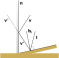
\includegraphics[width=0.4\textwidth]{figures/backvector.pdf}
    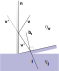
\includegraphics[width=0.4\textwidth]{figures/backvector_refract.pdf}
  \end{center}
  \caption{Geometry of the back-vector for reflection and refraction in MRM, illustrated in two dimensions. The view vector $\vecv$ is reflected in a ``virtual mirror'' to obtain $\vecvv$, which is then used to compute the half-vector with the light vector $\vecl$. The resulting back-vector ($\vecb_{r}$ for reflection and $\vecb_{t}$ for refraction) is used as microfacet normal selector.}
  \label{fig:backvector}
\end{figure}

As illustrated in Figure \ref{fig:backvector}, the reflection $\vecvv$ of the view direction $\vecv$ on the surface can also be interpreted as a reflection of the view direction in a ``virtual mirror'' aligned with $\vecv$ and perpendicular to the surface macronormal $\vecn$, thus turning glossy forward-reflection into glossy retroreflection.  \citet{BelcourBackvector} showed that this reflection is related to the geometry of double scattering on the microsurface. Though here there is no direct physical interpretation of the back-vector as such a scattering mode, this interpretation can serve as a motivation why the components of the regular microfacet model still work on changing the domain to the back-vector.

We now detail the mathematical consequences of using the back-vector as microfacet selector.

\paragraph*{Jacobian of Back-Vector.}
First we observe that the Jacobian of the change of variable from the back-vector to the light vector $\vecl$ for specular microfacets~(Equation~(11) and~(14) of \citet{WalterMicrofacet}) has the same form as the half-vector one:
\begin{equation}
\left\lVert \dfrac{\partial \omega_{\vecb_{r}}}{\partial \omega_{\vecl}} \right\rVert = \left\lVert \dfrac{\partial \omega_{\vech_{r}(\vecvv, \vecl)}}{\partial \omega_{\vecl}} \right\rVert = \dfrac{1}{4 \left| \vdot{\vecl}{\vech_{r}(\vecvv, \vecl)} \right|} = \dfrac{1}{4 \left| \vdot{\vecl}{\vecbr} \right|} \ .
\end{equation}
We also observe that this is true for refractive microfacets~(Equation (17) of \citet{WalterMicrofacet}):
\begin{equation}
\left\lVert \dfrac{\partial \omega_{\vecb_{t}}}{\partial \omega_{\vecl}} \right\rVert = \left\lVert \dfrac{\partial \omega_{\vech_{t}(\vecvv, \vecl)}}{\partial \omega_{\vecl}} \right\rVert = \dfrac{  \eta_o^2 \left| \vecl, \vech_{t}(\vecvv, \vecl)  \right|}{ \left\lVert \vech_{t}(\vecvv, \vecl) \right\rVert^2}
\end{equation}
This is due to the fact that we have to differentiate with respect to the light direction which is not altered by the back vector.

\paragraph*{Microfacet reflection term.}
There is experimental evidence~\cite{BelcourBackvector} that using a Fresnel term based on the back-vector can provide a good match to actual retroreflective material measurements for a reflection back-vector based BRDF.
As such, we update the formulation of $\rho(\vecv, \vecm)$~(Equation (11) of \citet{WalterMicrofacet}) to use the reflected view vector $\vecvv$ instead. From the aforementioned equivalence of the Jacobians, it follows that the reflection microsurface BRDF~(Equation (15) of \citet{WalterMicrofacet}) becomes
\begin{equation}
  f_r^m(\vecv, \vecl, \vecm) = F(\vecvv, \vecm) \dfrac{\delta(\vecb_r, \vecm) }{4 \left| \vdot{\vecvv}{\vecb_r} \right|^2}.
\end{equation}
We used the fact that $\left| \vdot{\vecl}{\vecb} \right| = \left| \vdot{\vecvv}{\vecb} \right|$.
Similarly, for the transmissive microsurface BTDF (Equation~(18) of \citet{WalterMicrofacet}) we get
\begin{equation}
  f_t^m(\vecv, \vecl, \vecm) = \left(1-F(\vecvv, \vecm)\right) \dfrac{\delta(\vecb_t, \vecm) \eta_o^2 }{\left( \eta_i \vdot{\vecv^\prime}{\vecb_t} + \eta_o \vdot{\vecl}{\vecb_t} \right)^2}.
\end{equation}
Thus for both reflection and refraction, the effect on the microsurface BSDF of using the back-vector as selector is to replace $\vecv$ by $\vecvv$ in the Fresnel term and in the denominators.

\paragraph*{Shadowing \& Masking.}
The term $G_{2}(\vecv,\vecl,\vechr)$ in the microfacet model accounts for shadowing and masking of microfacets.
\enlargethispage{1\baselineskip}
The shadowing-masking function $G_{2}(\vecv, \vecl, \vech)$ accounts for the geometrical occlusion of the incident and outgoing rays by the local microsurface geometry. It combines the visibility masking function $G_1(\vecv, \vech)$ for the view direction and the visibility shadowing function $G_1(\vecl, \vech)$ for the light direction: \footnote{This is the separable form commonly used in microfacet models; see Section 6 of \citet{HeitzMicrofacet} for a discussion of separable vs. non-separable shadowing-masking functions. In general, $G_{2}(\vecv, \vecl, \vech)$ is some function of $G_1(\vecv, \vech)$ and $G_1(\vecl, \vech)$, and thus reciprocity still holds.}
%In the case of independent shadowing and masking, it is common to use the separable form\footnote{See Section 6 of \citet{HeitzMicrofacet} for a discussion of separable vs. non-separable shadowing-masking functions. Our derivation holds for any valid $G_2$ function, but we focus here on the separable case for simplicity.}
\begin{equation}
G_{2}(\vecv, \vecl, \vech) = G_1(\vecv, \vech) \, G_1(\vecl, \vech)\ .
\end{equation}
%Mathematically, the BSDF is plausible if $G_{2}$ is symmetric w.r.t. to exchanging $\vecv$ and $\vecl$, fulfills
%$G_{2}(\vecv, \vech) \leq G_1(\vecv, \vecl)$, and if $G_1$ further establishes the correct projected area of visible microsurfaces \cite{HeitzMicrofacet}
%\begin{equation}\label{eq:visible}
%  \avdot{\vecv}{\vecn} = \int_{\Omega_{\vecv}} G_1(\vecv, \vech) \cldot{\vecv}{\vech} D(\vech) \diff\vech.
%\end{equation}
Popular choices for $G_1$
%with this property
are the Smith masking function
\begin{equation} \label{eq:smith_masking}
  G_{1,\text{Smith}}(\vecv, \vech) = \frac{\chi^+(\vdot{\vecv}{\vech})  \avdot{\vecv}{\vecn}}{\int_{\Omega_{\vecv}} \cldot{\vecv}{\vech} D(\vech) \diff\vech},
\end{equation}
where analytic expressions are available for Beckmann and GGX distributions, and the V-cavity masking function \cite{HeitzMicrofacet}
\begin{equation} \label{eq:vc_masking}
  G_{1,\text{VC}}(\vecv, \vech) =
  \min\left\lbrace\frac{2\avdot{\vecv}{\vecn}\avdot{\vecn}{\vech}}{\avdot{\vecv}{\vech}}, 1\right\rbrace,
\end{equation}
which is generally applicable for distributions with symmetry around the normal.

We assume Smith or V-cavity masking is applied to the mirrored microfacet distribution, and thus replace  $G_{2}(\vecv, \vecl, \vech)$  with $G_{2}(\vecvv, \vecl, \vech)$ in the retroreflective microfacet model. With Smith masking, this is actually identical to a regular microfacet BSDF, as $\vecvv$ and $\vecv$ share the same geometric configuration. For V-cavity masking, taking $\vecvv$ as view direction simply corresponds to selecting $\vecb$ as microfacet normal.
%\todo{\tiny Laurent: I think we could extract the shadowing from Matthias derivation here. The other way to justify the derivation of the full model is to highlight that Smith's shadowing/masking does not depend on the microfacet (appart from the sideness). Hence, whatever the microfacet selector (as long as the sideness matches), the shadowing/masking is the same. Since $\vecv$ and $\vecvv$ share the same slope, we can exchange them in the equation.}

\paragraph*{Final form.}
It follows from the above back-vector modifications that our MRM retroreflective model takes the trivial form of simply replacing $\vecv$ by $\vecvv$ in the original microfacet BRDF and BTDF expressions:
\begin{equation} \label{eq:retro_microfacet_model}
  %  f_\text{MRM}(\vecv, \vecl) = f(\vecvv, \vecl) = \frac{D(\vecb) \, G_{2}(\vecvv,\vecl) \, F(\vecvv, \vecb)}{4 \vdot{\vecvv}{\vecn} \vdot{\vecl}{\vecn}}
  f_\text{MRM}(\vecv, \vecl) =
  \begin{cases}
    f_{r, \text{MRM}}(\vecv, \vecl) = f_r(\vecvv, \vecl)  & \text{if \;} (\vdot{\vecv}{\vecn})(\vdot{\vecl}{\vecn}) \geq 0, \\
    f_{t, \text{MRM}}(\vecv, \vecl) = f_t(\vecvv, \vecl)  & \text{otherwise}.
  \end{cases}
\end{equation}
\begin{figure}[!tb]
  \centering
  \includegraphics[width=0.93\linewidth]{figures/brdf_plots.pdf}
  \caption{Comparison of the retroreflective MRM BRDF (blue) to the regular GGX microfacet BRDF (red) and rough-diffuse EON model (orange), as a function of view direction $\theta_o$ for fixed light directions $\theta_i \in \{45^\circ, 80^\circ\}$. The dashed lines are the roughness $0.1$ case, and the solid lines roughness $0.666$. The horizontal green line at $1/\pi$ is the Lambert BRDF.}
  \label{fig:brdf_plots}
\end{figure}

\paragraph*{BRDF comparison.}
To gain some quantitative insight into the behavior of the MRM model, Figure~\ref{fig:brdf_plots} plots the BRDF values of the MRM model (green) compared to the rough diffuse (albedo 1) EON model \cite{Portsmouth2025EON} (orange) and GGX (blue). For both MRM and GGX, the Fresnel factor is set to 1.
\enlargethispage{1\baselineskip}
The $0.1$ roughness case is a very strong, tight peak (note the logarithmic scale on the y-axis), while the $0.666$ roughness case is a much broader peak.
It is evident that MRM BRDF is the same as GGX,with the peak flipped to be back-scattering (at exactly $\theta_o =-\theta_i$, $\phi_o = \phi_i$).
The $\phi_o = 45^\circ$ case demonstrates the situation when the view direction is not aligned in the same azimuthal plane as the light direction. In this case. both GGX and MRM are dimmer than Lambert or EON, which compensates for the extra energy of the peaks of MRM and GGX (in which almost all of the energy is concentrated, in the reflection or retroreflection direction respectively for GGX and MRM).


\section{Plausibility of MRM}

We briefly show here that the retroreflective microfacet model of Equation~\eqref{eq:retro_microfacet_model} is physically plausible, i.e. that it fulfills reciprocity symmetry and energy conservation requirements.

\enlargethispage{0.5\baselineskip}

\subsection{Reciprocity}

\label{sec:reciprocity}

We first verify that the MRM microfacet model fulfills reciprocity symmetry, i.e. that:
\begin{equation}
  f_{\text{MRM}}(\vecv, \vecl) = f_{\text{MRM}}(\vecl, \vecv) \ , \quad f_{t,\text{MRM}}(\vecv, \vecl) = \frac{\etav^2}{\etal^2}f_{t,\text{MRM}}(\vecl, \vecv) \ .
\end{equation}
For brevity, in analogy to the notation for $\vecvv$ we generally let $\vecxx := \text{reflect}(\vecx, \vecn)$.
We will verify explicitly that the retroreflective model is symmetric under the interchange operation $(\vecvv, \vecl) \leftrightarrow (\vecll, \vecv)$, which is the equivalent of the usual reciprocity symmetry $(\vecv, \vecl) \leftrightarrow (\vecl, \vecv)$ for regular microfacet models.
Note that for this we will need to impose one technical assumption on the NDF $D$: we require that the microfacet normal distribution is reflection-symmetric around the normal (which is the case for all isotropic distributions and for anisotropic Phong, Beckmann, and GGX).

\paragraph*{NDF term.}

The NDF term $D(\vech)$ in the microfacet model selects the microfacets oriented with normal $\vech$. Under the interchange operation, we have to verify that
\begin{equation}
D(\vech(\vecvv, \vecl)) = D(\vech(\vecll, \vecv))
\end{equation}
for both reflection and refraction cases. Since $\vech(\vecvv, \vecl)$ is the reflection of $\vech(\vecll, \vecv)$ around the normal, this holds true if $D$ is reflection-symmetric around the normal, i.e. it takes the form
\begin{equation}
D(\vech) = D\left(\avdot{\vecn}{\vech}, \lvert \vdot{\mathbf{t_1}}{\vech} \rvert, \lvert \vdot{\mathbf{t_2}}{\vech} \rvert\right)
\end{equation}
which we as noted above is a requirement for our model, but true of most commonly used microfacet distributions (including for example anisotropic GGX).

\paragraph*{Shadowing \& Masking.}

The shadowing-masking function $G_{2}(\vecv,\vecl,\vech)$ in the microfacet model accounts for the geometrical occlusion of the incident and outgoing rays by the local microsurface geometry. We have to verify that
\begin{equation} \label{eq:shadowing_symmetry}
G_{2}(\vecvv,\vecl,\vech(\vecvv, \vecl)) = G_{2}(\vecll,\vecv,\vech(\vecll, \vecv)) \ .
\end{equation}
First, V-cavity masking manifestly satisfies the following symmetry under reflection of both the view and light directions \emph{and} the selected microfacet normal:
\begin{equation}
  G_2(\vecvv, \vecl, \vech(\vecvv, \vecl)) = G_2(\vecv, \vecll, \vech(\vecv, \vecll)) \ .
\end{equation}
as can be verified with Equation~\eqref{eq:vc_masking}. In the case of Smith masking, this also holds provided that $D$ is reflection-symmetric around the normal (which we assumed), as follows from Equation~\eqref{eq:smith_masking}. Then it follows from standard reciprocity that
\begin{equation}
  G_2(\vecv, \vecll, \vech(\vecv, \vecll)) = G_2(\vecll, \vecv, \vech(\vecll, \vecv)) \ .
\end{equation}
from which Equation~\eqref{eq:shadowing_symmetry} follows directly.

\paragraph*{Fresnel term.}

The Fresnel term $F(\vecv, \vech)$ in the microfacet model accounts for the proportion of light reflected vs. refracted at the microsurface. We have to verify that
\begin{equation}
F(\vecvv, \vech(\vecvv, \vecl)) = F(\vecll, \vech(\vecll, \vecv)) \ .
\end{equation}
Reflection symmetry of the Fresnel term implies
\begin{equation}
  F(\vecvv, \vech(\vecvv, \vecl)) = F(\vecv, \vech(\vecv, \vecll))
\end{equation}
and reciprocity symmetry further implies
\begin{equation}
  F(\vecv, \vech(\vecv, \vecll)) = F(\vecll, \vech(\vecll, \vecv)) \ .
\end{equation}
from which the desired equality follows.

\paragraph*{Summary.}

In summary, we can conclude the reciprocity symmetry of the BRDF
\begin{equation}
  f_{r,\text{MRM}}(\vecv, \vecl) = f_r(\vecvv, \vecl) =f_r(\vecll, \vecv) =  f_{r,\text{MRM}}(\vecl, \vecv).
\end{equation}
%\begin{equation}
%  \begin{split}
%  f_{r,\text{MRM}}(\vecv, \vecl) =
%  f_r(\vecvv, \vecl) &=
%  \frac{D(\vech(\vecvv, \vecl)) \, G_{2}(\vecvv, \vecl) \, F\left(\vecvv, \vech(\vecvv, \vecl)\right)}{4 \avdot{\vecvv}{\vecn} \avdot{\vecl}{\vecn} }\\
%  &=
%  \frac{D(\vech(\vecll, \vecv)) \, G_{2}(\vecll, \vecv) \, F\left(\vecll, \vech(\vecll,\vecv)\right)}{4 \avdot{\vecv}{\vecn} \avdot{\vecll}{\vecn} }\\
%  &=
%  f_r(\vecll, \vecv) =
%  f_{r,\text{MRM}}(\vecl, \vecv).
%  \end{split}
%\end{equation}
Analogously, we obtain the reciprocity symmetry requirement of the BTDF
\begin{equation}
    f_{t,\text{MRM}}(\vecv, \vecl) =  f_t(\vecvv, \vecl) = \frac{\etav^2}{\etal^2}f_t(\vecll, \vecv) = \frac{\etav^2}{\etal^2}f_{t,\text{MRM}}(\vecl, \vecv).
\end{equation}

%\begin{equation}
%  \begin{split}
%    &f_{t,\text{MRM}}(\vecv, \vecl)
%    =  f_t(\vecvv, \vecl)\\
%    &= \frac{\avdot{\vecvv}{\vecht(\vecvv, \vecl)}\avdot{\vecl}{\vecht(\vecvv, \vecl)}\etav^2 D(\vecht(\vecvv, \vecl)) \, G_{2}(\vecvv,\vecl) \, \left(1 - F(\vecvv, %\vecht(\vecvv, \vecl)) \right)}
%    {\avdot{\vecvv}{\vecn} \avdot{\vecl}{\vecn} \left(\etav \vdot{\vecvv}{\vecht(\vecvv, \vecl)} + \etal \vdot{\vecl}{\vecht(\vecvv, \vecl)}\right)^2} \\
%    &= \frac{\avdot{\vecv}{\vecht(\vecv, \vecll)}\avdot{\vecll}{\vecht(\vecv, \vecll)}\etav^2 D(\vecht(\vecll, \vecv)) \, G_{2}(\vecll,\vecv) \, \left(1 - F(\vecll, %\vecht(\vecll, \vecv)) \right)}
%    {\avdot{\vecv}{\vecn} \avdot{\vecll}{\vecn} \left(\etav \vdot{\vecv}{\vecht(\vecv, \vecll)} + \etal \vdot{\vecll}{\vecht(\vecv, \vecll)}\right)^2} \\
%    &=
%    \frac{\etav^2}{\etal^2}f_t(\vecll, \vecv) =
%    \frac{\etav^2}{\etal^2}f_{t,\text{MRM}}(\vecl, \vecv).
%  \end{split}
%\end{equation}

\subsection{Energy Conservation}

\label{sec:energy_conservation}

We now verify that the retroreflective microfacet model fulfills energy conservation, i.e. that the directional albedos fulfill
\begin{equation}
  \rho_{r, \text{MRM}}(\vecv) + \rho_{t, \text{MRM}}(\vecv) \leq 1.
\end{equation}
For the directional albedos we simply have
\begin{equation}
  \begin{split}
  \rho_{r, \text{MRM}}(\vecv) =
  \int_{\Omega_{\vecv}} f_{r, \text{MRM}}(\vecv, \vecl) \avdot{\vecl}{\vecn} \diff\vecl =
  \int_{\Omega_{\vecvv}} f_r(\vecvv, \vecl) \avdot{\vecl}{\vecn} \diff\vecl = \rho_r(\vecvv),\\
  \rho_{t, \text{MRM}}(\vecv) =
  \int_{\Omega_{-\vecv}} f_{t, \text{MRM}}(\vecv, \vecl) \avdot{\vecl}{\vecn} \diff\vecl =
  \int_{\Omega_{-\vecvv}} f_t(\vecvv, \vecl) \avdot{\vecl}{\vecn} \diff\vecl = \rho_t(\vecvv) \ .
  \end{split}
\end{equation}
That is, the directional albedo of MRM is equivalent to the directional albedo of the regular microfacet BSDF, but evaluated at the reflected direction.
As the original microfacet BSDF fulfills energy conversion, the retroreflective modification does, too.
%% Which, using equation \eqref{eq:visible} and $\frac{d\vech(\vecvv, \vecl)}{d\vecl} = \frac{1}{4 \vdot{\vecl}{\vech(\vecvv, \vecl)}}= \frac{1}{4 \vdot{\vecvv}{\vech(\vecvv, \vecl)}}$ \cite{WalterMicrofacet}, can be shown to fulfill energy conservation
%% \begin{equation}
%%   \begin{split}
%%   \rho(\vecvv) &=
%%   \int_\Omega \frac{D(\vech(\vecvv, \vecl)) G_{2}(\vecvv,\vecl)}{4 \vdot{\vecvv}{\vecn} \vdot{\vecl}{\vecn}}\vdot{\vecl}{\vecn} d\vecl\\
%%   &\leq
%%   \int_{\lbrace\vech \in \Omega: \vdot{\vecvv}{\vech} \geq 0\rbrace} \frac{D(\vech) G_1(\vecvv,\text{reflect}(\vecvv, \vech))}{\vdot{\vecvv}{\vecn}}\vdot{\vecvv}{\vech} d\vech
%%   = 1.
%%   \end{split}
%% \end{equation}
We further note that under our requirement of a reflection-symmetric microfacet normal distribution, the geometric
configurations for $\vecv$ and $\vecvv$ are identical.
Hence we can conclude $\rho_r(\vecv) = \rho_r(\vecvv)$ and $\rho_t(\vecv) = \rho_t(\vecvv)$, which in turn implies that the albedos of forward and retroreflection are the same, i.e. $\rho_{r, \text{MRM}}(\vecv) = \rho_r(\vecv)$ and $\rho_{t, \text{MRM}}(\vecv) = \rho_t(\vecv)$.


\section{Implementation Notes}
\label{sec:implementation}

Given an implementation of a regular microfacet BSDF, extending it to retroreflection is extremely straightforward (see the pseudo-code provided in Listing~\ref{lst:implementation}):

\begin{itemize}
\item
  Evaluation merely needs to replace $\vecv$ with $\vecvv$ upfront.
\item
  Similarly, importance sampling of $\vecl$ given $\vecv$ can be realized by replacing $\vecv$ with $\vecvv$ upfront and then importance sampling the regular microfacet BSDF.
  This may include low variance sampling using the domain of visible microfacets \cite{HeitzIS}.
\item
  As the albedos of standard BSDF and retroreflective BSDF are identical, compensating for the energy loss of microfacet single-scattering via a diffuse term \cite{KelemenBRDF, Kulla17} or normalization \cite{TurquinMultipleScattering} can thus be realized using the same data tables. The exact energy compensation of \citet{Heitz2016} can also be applied unchanged.
\item An implementation may optionally wish to provide a blend between regular and retroreflective microfacet behavior, to model materials with partial retroreflective properties (for example this is required in OpenPBR \cite{OpenPBR2024}). This can be achieved simply by blending $f_{r, \text{MRM}}$ and $f_r$, or alternatively via a stochastic selection (e.g. one-sample MIS \cite{Veach1998}) between the original $\vecv$ and reflected $\vecvv$ view directions during sampling.
\end{itemize}

%\noindent
\begin{lstlisting}[
    style=snippet,
    language=GLSL,
    caption=Pseudo code to implement the retroreflective microfacet model using an existing regular microfacet BSDF implementation,
    label=lst:implementation,
    nolol=true,
    frame=trBL
    ]
Sample_result sample_bsdf_retro(vec3 V, vec3 L, vec3 N, Bsdf_params params)
{
    vec3 Vp = -V + 2.0 * dot(V, N) * N;
    return sample_bsdf(Vp, L, N, params);
}

Eval_result eval_bsdf_retro(vec3 V, vec3 L, vec3 N, Bsdf_params params)
{
    vec3 Vp = -V + 2.0 * dot(V, N) * N;
    return eval_bsdf(Vp, L, N, params);
}
\end{lstlisting}

\newpage

\section{Results and Discussion}

\label{sec:results}

\paragraph*{Comparison to measured data}

\enlargethispage{0.5\baselineskip}

\begin{figure}[!t]
  \begin{center}
    \includegraphics[width=0.99\textwidth]{figures/brdf_theta_L_plots.pdf}
  \end{center}
  \vspace{-0.5cm}
  \caption{Measured BRDF of retroreflective tape (blue dots) at three different light source angles $\theta_L \in \{15^\circ, 30^\circ, 60^\circ\}$, and the MRM model fit (red line).}
  \label{fig:data_fit}
\end{figure}

\begin{figure}[!b]
  \centering
  \begin{tikzpicture}[font=\scriptsize ]
    \node[inner sep=1pt] (GGX0) {\includegraphics[width=0.3\linewidth,frame]{figures/conductor/cropped/classic_angle_0_cropped.png}};
    \node[inner sep=1pt,right = 0cm of GGX0] (GGX45) {\includegraphics[width=0.3\linewidth,frame]{figures/conductor/cropped/classic_angle_45_cropped.png}};
    \node[inner sep=1pt,right = 0cm of GGX45] (GGX90) {\includegraphics[width=0.3\linewidth,frame]{figures/conductor/cropped/classic_angle_90_cropped.png}};
    \node[inner sep=1pt,below = 0cm of GGX0] (MRM0) {\includegraphics[width=0.3\linewidth,frame]{figures/conductor/cropped/retro_angle_0_cropped.png}};
    \node[inner sep=1pt,right = 0cm of MRM0] (MRM45) {\includegraphics[width=0.3\linewidth,frame]{figures/conductor/cropped/retro_angle_45_cropped.png}};
    \node[inner sep=1pt,right = 0cm of MRM45] (MRM90) {\includegraphics[width=0.3\linewidth,frame]{figures/conductor/cropped/retro_angle_90_cropped.png}};
    \node[inner sep=1pt,above = 2pt of GGX0] { \textbf{$\Delta\theta_{vl}=0^\circ$} };
    \node[inner sep=1pt,above = 2pt of GGX45] { \textbf{$\Delta\theta_{vl}=45^\circ$} };
    \node[inner sep=1pt,above = 2pt of GGX90] { \textbf{$\Delta\theta_{vl}=90^\circ$} };
    \node[inner sep=1pt,left = 1pt of GGX0, anchor=south,rotate=90] { GGX };
    \node[inner sep=1pt,left = 1pt of MRM0, anchor=south,rotate=90] { MRM };
  \end{tikzpicture}
  \caption{Renders of a metallic shaderball with either a classic GGX (top row) or retroreflective MRM material (bottom row) applied, for various camera angles and a fixed light direction, with relative angle between the view and light direction $\Delta\theta_{vl} \in \{0^\circ, 45^\circ, 90^\circ\}$.}
  \label{fig:conductor_renders}
\end{figure}

\begin{figure}[!htb]
  \centering
  \begin{tikzpicture}[font=\scriptsize ]
    \node[inner sep=1pt] (Class1) {\includegraphics[width=0.3\linewidth,frame]{figures/dielectric/cropped/classic_ior_1_cropped_label.png }};
    \node[inner sep=1pt,right = 0cm of Class1] (MRM1) {\includegraphics[width=0.3\linewidth,frame]{figures/dielectric/cropped/retroRT_ior_1_cropped.png }};
    \node[inner sep=1pt,right = 0cm of MRM1] (Mixed1) {\includegraphics[width=0.3\linewidth,frame]{figures/dielectric/cropped/retroR_ior_1_cropped.png }};
    \node[inner sep=1pt,below = 0cm of Class1] (Class15) {\includegraphics[width=0.3\linewidth,frame]{figures/dielectric/cropped/classic_ior_1.5_cropped.png }};
    \node[inner sep=1pt,right = 0cm of Class15] (MRM15) {\includegraphics[width=0.3\linewidth,frame]{figures/dielectric/cropped/retroRT_ior_1.5_cropped.png }};
    \node[inner sep=1pt,right = 0cm of MRM15] (Mixed15) {\includegraphics[width=0.3\linewidth,frame]{figures/dielectric/cropped/retroR_ior_1.5_cropped.png }};
    \node[inner sep=1pt,above = 2pt of Class1] { \textbf{Classical Microfacet} };
    \node[inner sep=1pt,above = 2pt of MRM1] { \textbf{Full retroreflective MRM} };
    \node[inner sep=1pt,above = 11.5pt of Mixed1] { \textbf{Mixed MRM (BRDF)} };
    \node[inner sep=1pt,above = 0.5pt of Mixed1] { \textbf{and Classical (BTDF)} };
    \node[inner sep=1pt,left = 1pt of Class1, anchor=south,rotate=90] { $\mathbf{\boldsymbol{\eta} = 1}$ };
    \node[inner sep=1pt,left = 1pt of Class15, anchor=south,rotate=90] { $\mathbf{\boldsymbol{\eta} = 1.5}$ };
  \end{tikzpicture}
  \caption{Renders of a glass shaderball illuminated from the side. The index of refraction is $1.0$ (top) or $1.5$ (bottom). From left to right: classic microfacet BSDF (left), retroreflective BSDF (middle), and combined retroreflective BRDF and classic BTDF (right).  }
  \label{fig:dielectric_renders}
\end{figure}

Figure~\ref{fig:data_fit} shows a fit of the retroreflective MRM model (in red) to the measured BRDF of retroreflective tape (in blue) from \cite{BelcourBackvector}. This is the "yellow tape" sample from their dataset, illuminated at three different light source angles $\theta_L \in \{15^\circ, 30^\circ, 60^\circ\}$ (in the plane of incidence).  The MRM model provides a reasonably good match to the retroreflective peak using a roughness of $r = 0.23$, together with ``F82-tint'' Fresnel \cite{OpenPBR2024} with $F_0=0.19$ and $F_{82} = 0$.

\paragraph*{Incorporation in a standard microfacet model}

Figure~\ref{fig:conductor_renders} shows renders of a shaderball with either a classic GGX or retroreflective MRM material applied, here assuming \emph{conducting} (i.e. metallic) microfacets.

\paragraph*{Combination of BRDF and BTDF}

The albedo is identical for forward- and retroreflective BRDF as well as BTDF, which allows to arbitrarily combine forward- and retroreflective variants into a BSDF. When constructing an artist-controllable retroreflective dielectric BSDF, we observed that using $f_t$ instead of $f_{t, \text{MRM}}$ yields more intuitive results, in particular for an index of refraction close to 1. An implementation could reasonably choose either this formulation or the full retroreflective BTDF, depending on the desired effect.

Figure~\ref{fig:dielectric_renders} demonstrates this in renders of a dielectric shaderball, where the IOR of the dielectric material is either $1.0$ (top row) or $1.5$ (bottom row).
Left to right we show three combinations of BRDF and BTDF: the classic microfacet BSDF $f_r$ and BTDF $f_t$ (left), the retroreflective BRDF $f_{r,\text{MRM}}$ plus retroreflective BTDF $f_{t,\text{MRM}}$ (middle), and retroreflective BRDF $f_{r,\text{MRM}}$ combined with the classic (non-retroreflective) BTDF $f_t$ (right).



\section{Conclusion}

We have presented a retroreflective microfacet model (MRM) based on a simple modification of the classic microfacet BSDF. We have shown that the model fulfills reciprocity and energy conservation requirements, making it a physically plausible microfacet model. This model can be used to represent materials with strong retroreflective properties, such as certain fabrics or retroreflective coatings,  with a reasonable degree of accuracy and very efficiently. The model is straightforward to implement in existing renderers supporting microfacet BSDFs, as it only requires reflecting the view direction about the surface normal before evaluating the standard microfacet model.

Due to its simplicity and ease of integration into existing microfacet-based rendering systems, the MRM model has been proposed as a standard component in the OpenPBR material model \cite{OpenPBR2024} (and correspondingly in the MaterialX modeling framework \cite{Smythe2016}).

\small

\bibliographystyle{jcgt}
\bibliography{citations}

\section*{Author Contact Information}

\hspace{-2mm}\begin{tabular}{p{0.48\textwidth}p{0.48\textwidth}}
Matthias Raab \newline
\href{mailto:mraab@nvidia.com}{mraab@nvidia.com} \newline
&
Laurent Belcour \newline
\href{mailto:laurent.belcour@gmail.com}{laurent.belcour@gmail.com} \\
Frankie Liu \newline
\href{mailto:frankie.liu@gmail.com}{frankie.liu@gmail.com} \newline
&
Jamie Portsmouth \newline
\href{mailto:jamports@mac.com}{jamports@mac.com} \newline
\end{tabular}


\end{document}


